\documentclass{article}
%\documentclass[a4paper,12pt,times,numbered,print,index]{Class/ThesisPDF}
\usepackage[utf8]{inputenc}
\usepackage{geometry}
\usepackage{amsmath}
\usepackage{xcolor}
\usepackage{multicol}
\usepackage{graphicx}
\usepackage{titlesec}
\usepackage[english]{babel}
\usepackage{listings}
\usepackage{minted}
\usepackage{algorithm}
\usepackage[noend]{algpseudocode}
\usepackage{subcaption}
\usepackage[english]{babel}
\usepackage[
backend=biber,
style=alphabetic,
sorting=ynt
]{biblatex}

\setlength{\columnsep}{0.5cm}
\geometry{a4paper,left=3cm,right=3cm,top=3cm,bottom=4cm}
\addbibresource{reference.bib}
%%----------------- Settings ----------------------%%
%\addbibresource{bib/reference.bib}

\begin{document}


\begin{titlepage}
    \begin{center}
        
\includegraphics[width=0.5\textwidth]{pic/Bham_withname.jpg}
        \vspace*{2cm}
 
        \Huge
        \textbf{Solving Bayesian Inference with Weighted Model Counting}
 
        \vspace{0.5cm}
        
        \vspace{1.5cm}
        \Large
        \textbf{Tianyang Sun}
 
        \vspace{2.5cm}
 
        BSc. Computer Science
 
        \vspace{1.0 cm}
 
        \Large
        School of Computer Science\\
        University of Birmingham\\
        April 2019
 
    \end{center}
\end{titlepage}

\begin{abstract}
    This report introduces the propositional encoding of Bayesian Networks that reduce the Bayesian inference to Weighted Model Counting. The approach encode Bayesian networks into conjunctive normal forms (CNFs) that are associate with weights, and compute the sum of weights of the model that the variables are consistent with the evidence.
     Our work implemented four CNF encoding schemes and tested the performance by feeding the encoded CNFs into the model counter miniC2D, and used runtime and file size for evaluation.\\
     
     \noindent The project can be found on \url{https://github.com/txs799/Project} \\
     
     \noindent \textit{\textbf{Key words:}} Bayesian Networks, Exact Bayesian Inference, Weighted Model Counting
     
\end{abstract}

\newpage
\section*{Acknowledgments}
\text{red}{Insert Acknowledgements Here}

\newpage
\tableofcontents
\newpage


\section{Introduction}
    \subsection{Motivation}
    Bayesian networks are widely used to model uncertainty by assigning probabilities to every possible states. It allows modeling large scale variables and represent models with a network.
    Bayesian inference is based on solid rules of probability calculus such that all the assumptions are contained in the model.
    Probablistic inference is that, given observations of some model variables, compute the posterior probabilities. it is widely used in game theory, statbility testing and medical diagnosis. 
    % why exact inference
    Bayesian inference consists of exact inference and approximate inference, for exact inference....\par
    There are some existing methods for performing exact Bayesian inference, including...
    Some common methods for exact inference are Variable elimination and junction tree algorithms, while for some large scale bayesian networks, bayesian networks are time consuming. In \cite{enc1}, Mark charvia et al, presented a method which perform Bayesian inference with Weighted Model Counting by encoding Bayesian networks into logic forms. This encoding method can also be used to encode other probabilitic graphical models such as Markov chains, and performing weighted model counting has been experimented to outperform junction tree algorithm for the Bayesisn networks that has large determinism.\par
    
    \subsection{Project Aims}
    The goals of this project are listed below:
    \begin{itemize}
        \item Understand both Bayesian Networks and Weighted Model Counting.
        \item Explore and compare the existing encoding algorithms that encode Bayesian Networks to Conjunctive Normal Forms.
        \item Explore different Model Counting tools.
        \item Implemented three encoding schemes in \cite{enc1,enc2,2006-enc3}.
        \item Experiment the encoding schemes by encoding both benchmarks and real examples.
        \item Evaluate the performance of the encoding schemes by feeding the encoding output to the model counter.
    \end{itemize}

    \subsection{The structure of the report}
    The structure of the report follows:


\newpage

\newpage
\section{Background Knowledge}
This section will first introduce Bayesian Network and Bayesian inference, then, it will introduce logic normal forms, and several other concepts to aid the understanding of the later sections.
    \subsection{Bayesian Network}
    The variable domain in this report refers to finite domains. The definition of the Bayesian network is from \cite{2008-literature-review}\\
    \begin{itemize}
        \item instantiation: An instantiation of a set of Variables \textbf{X} is an assignment to each $X \in$ \textbf{X} of the value within the domain of X.
        \item Joint distribution over \textbf{X} is the probability function F that map the instantiation to the value in [0, 1], The $\Sigma$ F(X) = 1.
        \item factor: factors are functions that can represent in different ways. In bayesian networks, factor is simply the Conditional Probability Tables (CPT).
    \end{itemize}
    \textbf{Bayesian networks} are probabilistic models (G, P) that specify joint probability distributions. G denotes the directed acylic graphs (DAG), and P denotes the set of factors. For each node \textit{X} with random variables $\{x_{1}, ... x_{m}\}$ and its a parents \textit{Y}, there's a conditional probability distribution $P(x_{i}|Y)$. \\
    
    \noindent The joint probability distribution of the Bayesian network: 
    $$P(x_{1}, ... , x_{m}) = \Pi_{i = 1}^{m} P(x_{i}|Y)$$
    $$P(x_{1},.., x_{m}) = \Pi_{i = 1}^{m}P(x_{i}|x_{i - 1}, .. x_{1})$$
    So Bayesian networks assume that given values of parents of a network variable $X$, $X$ is independent of all its other predecessor variables in the graph and it can be written as: $$P(x_{i}|x_{i- 1}, ..., x_{1}) = P(x_{i}|Y)$$
    
    \noindent The Conditional distributions $P(X|Y)$ are obtained as follow:
    $$P(X|Y) = \frac{P(X,Y)}{P(X)}$$
    An example of a Bayesian Network called Asia.net from bnlearn repository is given in Figure 
    
    \begin{figure}
        \centering
        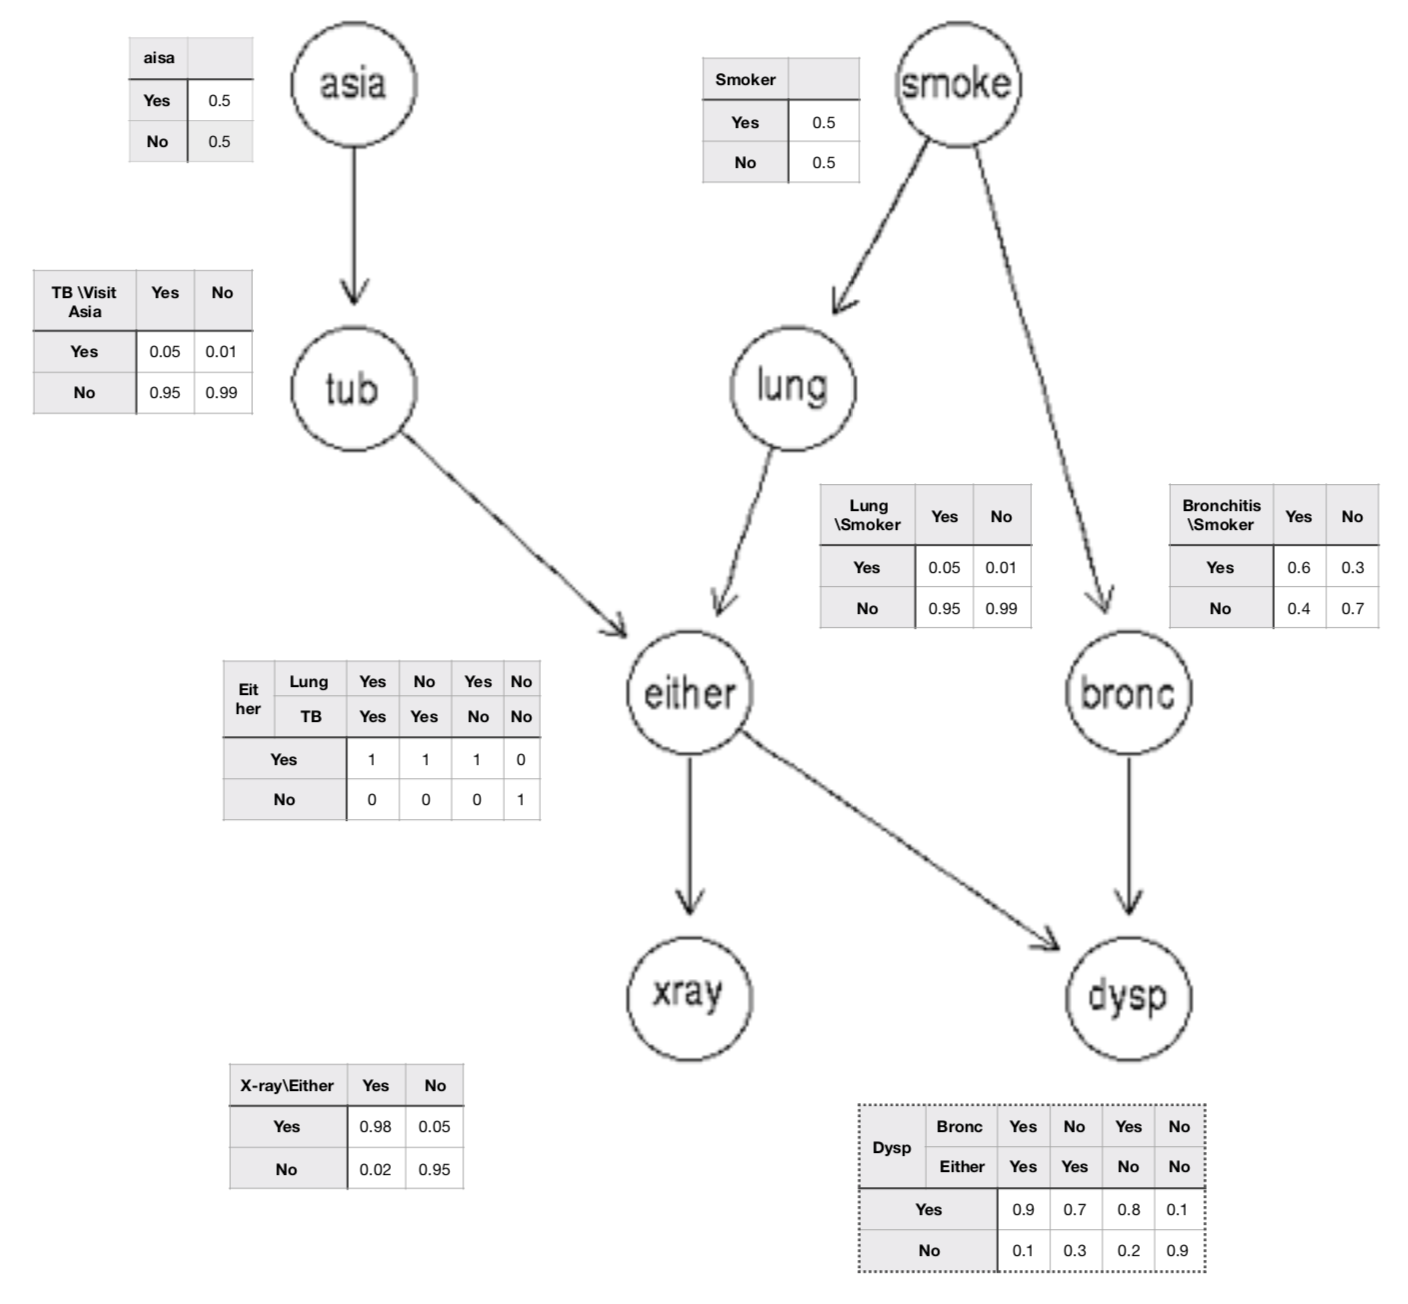
\includegraphics[width = 0.7\textwidth]{pic/full-asia.png}
        \caption{An example Bayesian network Asia.net modeling the toy process of diagnosing lung canber}
        \label{fig:asia-net}
    \end{figure}
    
    \subsection{Exact Bayesian Inference}
    % Given a Joint density for X = $(X_{i}, i \in V)$ of the following form:
    % $$p(u) = \frac{1}{Z} \Pi_{c \in C} \Phi_{c}(u_(c))$$
    % Compute the marginal density of $X_{Q}$:
    % $$p_{q}(v) = \Sigma_{u \in X_{\bar{Q}}} \frac{1}{Z} \Pi_{c \in C} \Phi_{C}(v_{c} \cup u_{c})$$
    Given an Bayesian Network BN over Variables ${X, Y...}$. and probability distributions \textbf{Pr}. There are three reasonable questions to ask regarding the probability distributions:
    \begin{itemize}
        \item What is the most likely instantiation of network variables X given some evidence \textbf{e}
        $$MPE(e) = argmax_{x} Pr(x, e)$$
        \item What is the probability of an evidence \textbf{e}.
        \item What is the assignment y over the complete variables that maximize $P(y|x)$ given an evidence \textbf{x}
    \end{itemize}
    \subsection{Multi\-linear functions}
    A \textit{multi\-linear function} over variables $\Sigma$ is a function
    with the form $t_{1} + t_{2} + ... + t_{n}$ in which each term $t_{i}$ is a product of some distinct variables. \\
    $\Sigma = \lambda_{x}, \lambda_{y}, \lambda_{z}, \theta_{1}, \theta_{2}, \theta_{3}$, an example of muti\-linear function: $f = \lambda_{x}\theta_{1} + \lambda_{y}\theta_{2} + \lambda_{z}\theta_{3}\theta_{2}$\\
    
    \noindent In the project, the idea of CNF encoding of Bayesian networks is to represent the Bayesian network with multi-linear function and then perform the encoding.
    
    \subsection{Normal Forms}
    \textbf{Conjunctive Normal Forms}\\
    
    \noindent In boolean logic, a clause that contains only $\vee$ is called \textbf{disjunctive clause}, and a clause contains only $\wedge$ is called \textbf{Conjunctive clause}.\\
    Conjunctive Normal Forms (also written as clausual normal form) is  the conjunction (\textit{AND}) of one or several clauses, and is a disjunction (\textit{OR}) of literals. An example is given below: $$(p \vee q \vee \neg r) \wedge (\neg q \vee s)$$
    
    \noindent \textbf{Negation Normal Forms}\\
    
    \noindent A formula is in \textbf{negation normal form}  (NNF) if the negation operator is only applied to variables and the only other allowed operators are conjunction (AND) and disjunction (OR).\\
    \newpage
    \noindent \textbf{Decomposability, Determinism Negation Normal Form}\\
    
    \begin{itemize}
        \item \textbf{Decomposibility}: In an NNF, for any two children $node_{i}$ and $node_{j}$, and any node \textit{n} $Variables(node_{i}) \cap Variabes(node_{j}) = \emptyset$.
        \item \textbf{determinism}: In an NNF, for any two children $n_{i} \wedge n_{j}$ is logically inconsistent for any node connected by \textbf{\textit{or}}.
        \item \textbf{Smoothness}: In an NNF, for each disjunction C in the NNF, $C_{1}, ... C_{n}$ mentioens the same variables.
    \end{itemize}
    
    \noindent Three figures of examples are given in \cite{2002language-map} to show these properties, shown in Figure \ref{fig:demo-DDNNF}.
    \begin{figure}
        \centering
        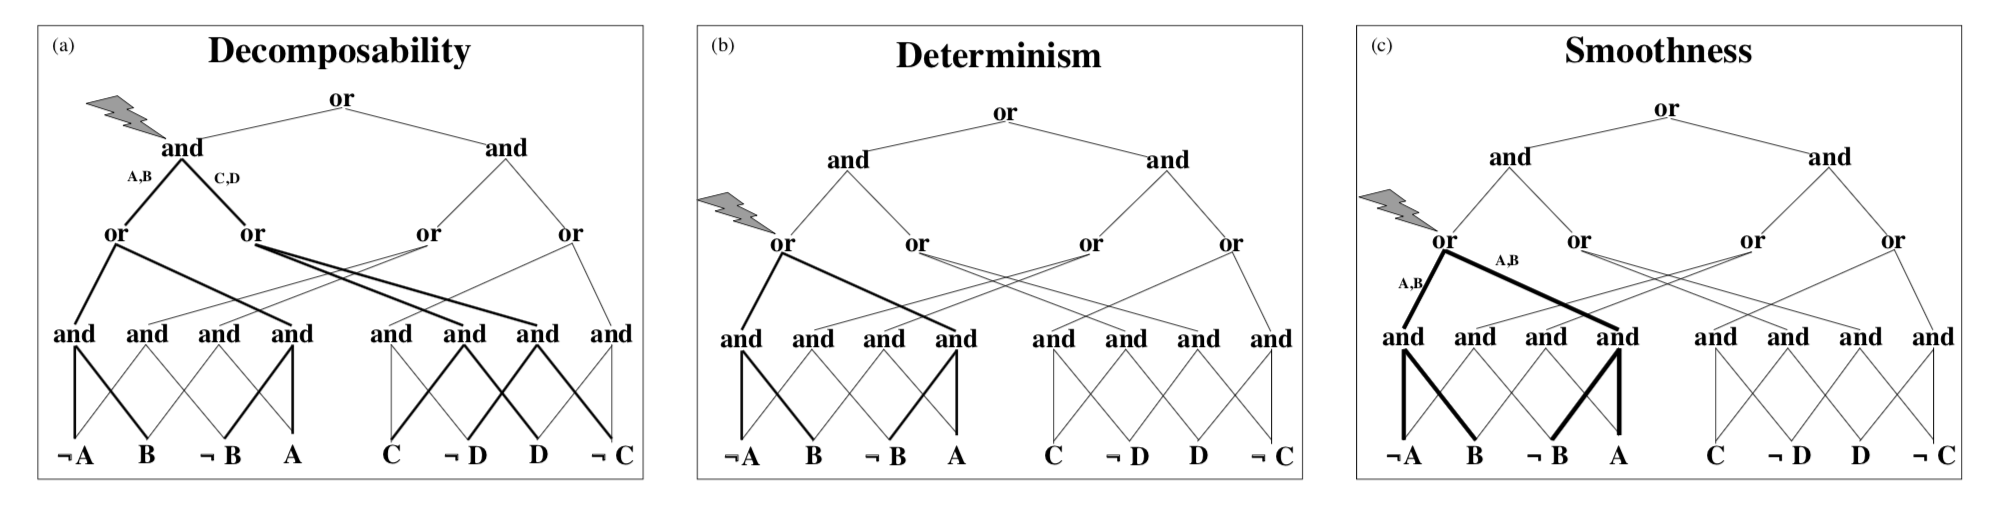
\includegraphics[width = 0.8\textwidth]{pic/DDNNF.png}
        \caption{The example which demonstrate the property of Decomposiblity, Determinism and Smoothness of a NNF given in \cite{2002language-map}}
        \label{fig:demo-DDNNF}
    \end{figure}
    
    \subsection{DPLL}
    Davis–Putnam–Logemann–Loveland (DPLL) algorithm is a complete, backtracking-based search algorithm for deciding the satisfiability of propositional logic formula in conjunctive normal forms \cite{Davis:1960:CPQ:321033.321034}. The algorithm runs by assigning a truth value to a chosen literal to simplify the formula then check satisfiablity recursively.\\ 
    \noindent \textbf{Unit propagation}:\\
    \noindent If a clause contains only one single literal that is not assigned, assign the value that make this literal true.\\
    \noindent \textbf{Pure literal elimination}:\\
    \noindent If a formula contains a propositional variable with only one polarity, remove all the clauses that contains the variable.\\
    
    \noindent The DPLL algorithm is described below based on \cite{DPLLbook}:
    \begin{lstlisting}[mathescape]
    function DPLL($\Phi$)
       if $\Phi$ is a consistent set of literals
           return true;
       if $\Phi$ contains empty clause
           return false;
       for every unit clause {l} in $\Phi$
          $\Phi$ <-  unit-propagate(l, $\Phi$);
       for every literal l that occurs pure in $\Phi$
          $\Phi$  <- pure-literal-assign(l, $\Phi$);
       l gets choose-literal($\Phi$);
       return DPLL($\Phi$ $\wedge$ {l}) or DPLL($\Phi$ $\wedge$ {$\neg$ (l)});
    \end{lstlisting}
    
   
    \subsection{Sensitional Decision Diagram}
    According to \cite{Darwiche:2011:SNC:2283516.2283536}, Sensitional Decision Diagram (SDD) is a Boolean function F(X,Y) which can always be decomposed into the following format:
    $$f(\textbf{X, Y}) = (p_{1}(X) \wedge s_{1}(Y)) \vee (p_{n}(X) \wedge s_{n}(Y)) $$
    The X and Y are disjoint set that $X \wedge Y = \emptyset$ and the decomposition satisfies the \textbf{X-Y partition}. It has been shown in \cite{Darwiche:2011:SNC:2283516.2283536} that it is a traceable representation of Boolean function.
    \textbf{X-Y partition} holds if the decomposition of the boolean function satisfy the following:
    \begin{itemize}
        \item  $\forall$ i, $p_{i} \neq FALSE$;
        \item for $i \neq j$, $p_{i} \wedge p_{j} = FALSE$
        \item $p_{1} \vee ... \vee p_{n} = TRUE$
    \end{itemize}
    
    \subsection{Propositional Model Counting}
    Propositional Model counting is the problem of counting the number of models for a certain propositional formula.\cite{Biere:2009:HSV:1550723-sat-handbook} That is, counting the number of unique assignment that make the formula TRUE. This problem can be solved by exploiting DPLL and local search algorithms.
    
    \subsection{Deterministic Belief network}
    Belief networks which have 0/1 parameters, except possibly for the parameters of root variables, are known as deterministic belief networks.\cite{enc1}
    
    
    

\newpage
\section{Literature Review}
In this section, the related work are discussed in the following dimensions:
\begin{enumerate}
    \item Exact Bayesian inference methods.
    \item Several encoding schemes that can reduce the computation of probability of the evidence for a Bayesian Network into a Weighted model counting problem. 
    \item Exisiting model counting tools.
\end{enumerate}
    \subsection{Bayesian inference methods}
        \subsubsection{Variable Elimination}
        Variable Elimination is a Exact inference method. The idea is to exploit the structure by eliminating the non-observed and non-queried variables once at a time.\\
        
       \noindent A Factor is a function from a tuple of random variables to a number, denoted by $f(X_{1}, X_{2}, ... , X_{j})$, it denotes a distribution over $\{X_{1}, .., X_{j}\}$. 
        \begin{itemize}
            \item  By assigning some of (or all of) the variables in a factor, new factors can be made out of an existing factor. For example: $f(X_{1} = v_{1}, X_{2}, ..., X_{j})$ is a factor of $\{X_{2}, ... , X_{j}\}$ when $v_{1}$ is assigned to $X_{1}$.
            \item A variable can be signed out. Consider the $X_{1}$ over domain $\{v_{1}, .. ,v_{m}\}$, the variable $X_{1}$ can be summed out with the formula below: $$\Sigma_{i= 1}^{m}f(X1 = v_{i}, X_{2}, ..., X_{j})$$
            \item Factors can be multiplied. Consider two factors $f_{1}(X_{1}, X_{2}, X_{3})$ and $f_{2}(X_{1}, X_{4}, X_{5})$ which they both have $X_{2}$ in common. A new factor is defined below: $$(f_{1} \times f_{2})(X_{1}, .. X_{5}) = f_{1}(X_{1}, X_{2}, X_{3}) \times f_{2}(X_{1}, X_{4}, X_{5}) $$
        \end{itemize}
        
        \noindent Given variables over a Bayesian Network $X_{1}, ... , X_{m}$, the factor $P(Z, Y_{1}=v_{1}, ... , Y_{j}= v_{j})$ can be computed by summing out $Z_{1}, ..., Z_{k} =  \frac{\{X_{1}, ... X_{n}\}}{Z, Y_{1}, ..., Y_{j}}$.\\
        
        \noindent Given the factors $P(X_{i}|iX_{i})$ and chain rule, $P(X_{1}, ..., X_{n})$ can be written as: $\Pi_{i = 1}^{n} P(X_{i}|pX_{i})$. So we have:
        $$P(Z, Y_{1}=v_{1}, ... , Y_{j}= v_{j}) = \Sigma_{Z_{k}}.. \Sigma_{Z_{1}} \Pi P(X_{i}|pX{i})_{Y_{1} = v1, .. Y_{j} = v_{j}}$$
        
       
        \noindent To sum up, the Variable elimination algorithm is to repeat
        \begin{enumerate}
            \item choose a variable to eliminate.
            \item push in its sum as far as possible.
            \item Compute the sum to result in a new factor.
        \end{enumerate}
        \newpage
        \noindent \textbf{Complexity of Variable Elimination}\\
        
        \noindent The time and space complexities of Bayesian inference with Variable Elimination algorithm depends on the size of the largest intermediate factor. It is a NP-hard problem to choose the elimination order that minimize the complexity.\\
        
        \noindent The Variable Elimination is also query sensitive, that is the query variables should be specified in advance. Each time we run a diffenerent query, we must re-run the entire algorithm.
        
        \subsubsection{Junction tree}
        Junction tree algorithm, or sometimes called Joint tree algorithm is another exact Bayesian inference algorithm. This algorithm generalize Variable Elimination to deal with the query sensitive problem. It can execute a large number of queried simultaneously.\\
        
        \noindent \textbf{Define a junction tree:}\\
        
        The cluster graph T is a junction tree is it satisfy the following three properties:
        
        \begin{enumerate}
            \item \textbf{Single connectivity:} A cluster graph satisfy singly connectivity if there is one and only one path connecting between each cluster.
            \item \textbf{Covering:} A cluster graph satisfy covering if got each clique A of G, there is some cluster C such that A $\subseteq$ C.
            \item \textbf{Running intersection:}  A cluster graph satisfy  running intersection if for each pair of clusters B and C that both contain \textit{x}, the cluster between the unique path connecting B and C also contains \textit{x}.
        \end{enumerate}
        
        \noindent To build a junction tree, first choose an order of nodes and perform Variable elimination to obtain elimination cliques, then build the complete cluster graph over the maximum elimination cliques, after that, weight the edges and compute the maximum weight juntion tree.
        Figure \ref{fig:bayesjunc} shows a Bayesian network and its corresponding junction tree with the assignment of the factors.\\
        
        \begin{figure}
            \centering
            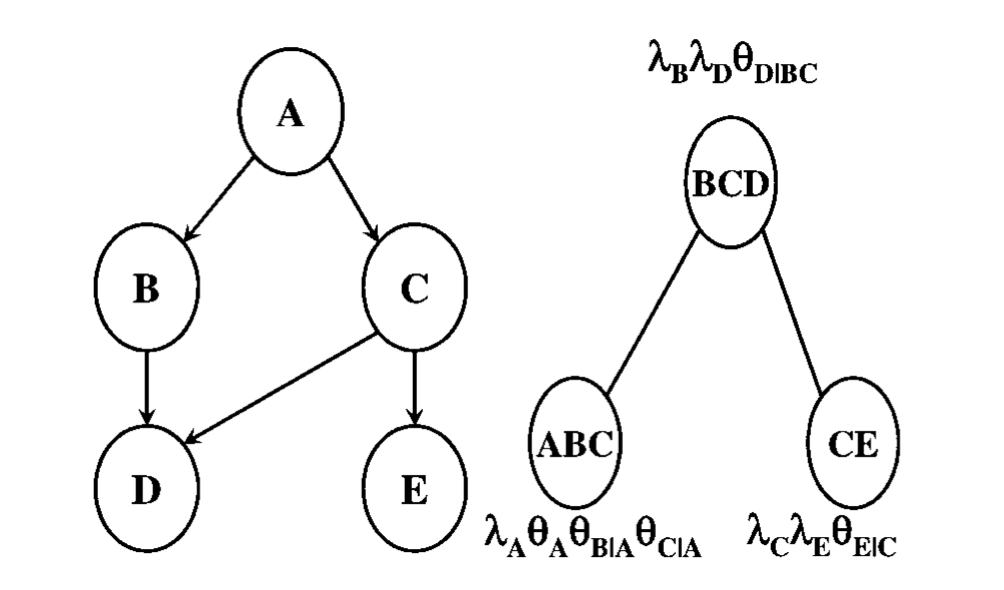
\includegraphics[width = 0.6\textwidth, height = 0.3\textwidth]{pic/bayesandjunctree.png}
            \caption{Left A Bayesian network, Right: its corresponding junction tree}
            \label{fig:bayesjunc}
        \end{figure}
        
        \noindent \textbf{Complexety of junction tree algorithm}\\
        
        \noindent Junction tree algorithm can be viewed as a decent way of performing Variable elimination. Different elimination orders will lead to different junction trees and finding the junction tree that have the smallest cluster is a NP-hard problem.\\
        
        \noindent The time and space complexity is dominated by the size of the largest cluster in the junction tree. The complexity with tabular density Bayesian Networks is \textbf{exponential} in the size of the largest cluster.
        
        
        %%% 还没写完
        \subsubsection{Weighted model Counting}
        To perform Bayesian Inference with Weighted model counting, the Bayesian networks are represented as multi\-linear functions and encoded into Conjunctive Normal Forms (CNF) and feed the CNFs are feed into Model Counters. The section below describes several encoding schemes to perform Weighted model counting method, and also review several existing model counters.
    
    \subsection{Encoding Bayed to CNF}
        \subsubsection{Full encoding}
            \textbf{Generating CNFs}
            \newline
            Given a Bayesian Network, two types of variables are generated.
            Define the variables generated from Node \textbf{\textit{X}} as Indicator Variables.
            For a node \textbf{\textit{X}} in Bayesian Network \textbf{N}, let $\lambda_x$ define the indicator variable. 
            Define the variables generated form Node \textbf{\textit{X}} and its parents \textbf{Y} = {$Y_{1}$, ... $Y_{n}$} as Parameter Variables.
            For a node \textbf{\textit{X}} in Bayesian Network \textbf{N}, let $\theta_{X|Y}$ denotes the parameter variable.\\
            
            \noindent \textbf{Obtaining indicator clauses \textsc{I}:}\\
            For each node \textit{X} in a Bayesian Network with probability \{$x_{1}$,... ,$x_{n}$\} $\in$ \textit{X}, the following clauses are generated:
            % Indicator Clauses and Parameter Clauses
            \begin{equation}\label{fullenc_ic1}
                \lambda_{x_{1}} \vee ... \vee \lambda_{x_{n}}
            \end{equation}
            
            \begin{equation}\label{eq:fullenc_ic2}
                \neg\lambda_{x_{i}} \vee \neg\lambda_{x_{j}}, \;\;\; \mbox{for each i $\neq$ j}
            \end{equation}
            According to the commutation of logic OR, $R \vee Q$ $\Longleftrightarrow$ $Q \vee R$, to avoid redundant clauses, \ref{eq:fullenc_ic2} can be simplified as :
            \begin{equation}\label{fullenc_ic3}
                \neg\lambda_{x_{i}} \vee \neg\lambda_{x_{j}}, \;\;\; \mbox{for each i $<$ j}
            \end{equation}
            
            % parameter clauses
            \noindent \textbf{Obtaining parameter clauses \textsc{P}:}\\
            For each node \textbf{\textit{X}} in a Bayesian Network and its parents \textbf{\textit{Y}}, the following clauses are generated:
            \begin{equation}\label{fullenc_pc1}
                \lambda_{x_{i}} \wedge \lambda_{y_{1}} \wedge... \wedge \lambda_{y_{m}} \leftrightarrow \theta_{x_{i}|y_{1}..y{m}}
            \end{equation}
            
            % parameter clauses
            The following equation is the equivalent of \ref{fullenc_pc1} written in the way that meet the requirement of CNF.
            \begin{equation}\label{fullenc_IP}
                \neg\lambda_{x_{i}} \vee \neg\lambda_{y_{1}} \vee... \vee \neg\lambda_{y_{m}} \vee \theta_{x_{i}|y_{1}..y_{m}}
            \end{equation}
            \begin{equation}\label{fullenc_PI}
                \neg\theta_{x_{i}|y_{1}..y_{m}} \vee \lambda_{x_{i}},\\ \;\;
                \neg\theta_{x_{i}|y_{1}..y_{m}} \vee \lambda_{y_{j}} \;\; \mbox{ j = 1, ..., m}
            \end{equation}
            An example is given below from, consider a Bayesian network 'Asia', figure \ref{fig:asia-tub} shows two of the nodes 'asia' and 'tub'.
            
            \begin{figure}[h]
            \centering
            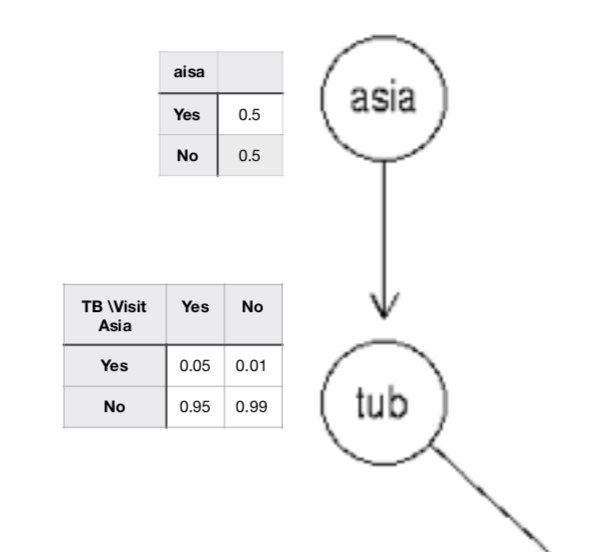
\includegraphics[width=0.25\textwidth]{pic/asia-tub.png}
            \caption{Two nodes from Asia Bayesian network}
            \label{fig:asia-tub}
            \end{figure}
            %% Here should be the example with BN asia
            \newpage
            \begin{multicols}{2}
            [
            \noindent The following clauses are generated for Node aisa and Node TB:
            ]
            \noindent \textbf{Node asia} = \{$Visit\_asia_{yes}$, $Visit\_asia_{no}$\}\\
            \newline
            \textbf{Indicator clauses:}\\
            $\lambda_{asia_{Y}} \vee \lambda_{asia_{N}}$\\
            $\neg \lambda_{asia_{Y}} \vee \neg\lambda_{asia_{N}}$\\
            \newline
            \textbf{Parameter clauses:}\\
            $\lambda_{asia_{Y}} \rightarrow \theta_{asia_{Y}}$\\
            $\theta_{asia_{Y}} \rightarrow \lambda_{asia_{Y}}$\\
            %%% fen ge xian %%%
            
            \columnbreak
            \noindent \textbf{Node TB} = $\{Tubercolosis_{yes}, Tubercolosis_{no}\}$:\\
            \newline
            \textbf{Indicator clauses:}\\
            $\lambda_{TB_{Y}} \vee \lambda_{TB_{N}}$\\
            $\neg \lambda_{TB_{Y}} \vee \neg\lambda_{TB_{N}}$\\
            \newline
            \textbf{Parameter clauses:}\\
            $\lambda_{TB_{Y}} \wedge \lambda_{asia_{Y}}\rightarrow \theta_{TB_{Y}|asia_{Y}}$\\
            $\theta_{TB_{Y}|asia_{Y}} \rightarrow \lambda_{TB_{Y}}$\\
            $\theta_{TB_{Y}|asia_{Y}} \rightarrow \lambda_{asia_{Y}}$\\
            $\lambda_{TB_{N}} \wedge \lambda_{asia_{Y}} \rightarrow \theta_{TB_{N}|asia_{Y}}$\\
            $\theta_{TB_{N}|asia_{Y}} \rightarrow \lambda_{TB_{N}}$\\
            $\theta_{TB_{N}|asia_{Y}} \rightarrow \lambda_{asia_{Y}}$\\
            \end{multicols}
            
        \subsubsection{Simplified full encoding}
        \textbf{Nodes with cardinality = 2}\\
        Now consider the node with cardinality 2. Take an Example in asia network, in figure \ref{fig:asia-tub} node \textit{asia} has two possibilty \textit{Yes} and \textit{No}, so according to \ref{fullenc_ic1}, we have $\lambda_{Visitaisa_{yes}} \vee \lambda_{Visitaisa_{no}}$ and this will always be 1, and the same apply for $\neg\lambda_{Visitaisa_{yes}} \vee \neg\lambda_{Visitaisa_{no}}$ \\
        \newline
        \noindent \textit{Simplification step 1:} If the cardinality of a node in a Bayesian Network is 2, ommit the clause in formula \ref{fullenc_ic1} and formula \ref{fullenc_ic3} in \textit{3.2.1 Full Encoding}.
        \newline
        
        \noindent \textbf{Encoding deterministic:}\\
        Now take a closer look at the values in each CPT, the deterministic can be captured.\\
        
        \noindent \textit{Simplification step 2:} When the parameter variable $\theta_{x_{i}|y_{1}..y_{m}}$ = 0, the parameter clause \textbf{P} described by \ref{fullenc_pc1} can be written as a single clause: $$\neg\lambda_{x_{i}} \vee \neg\lambda_{y_{1}} \vee... \vee \neg\lambda_{y_{m}}.$$
        
        \noindent \cite{enc1} gives the explanation of this step: If network variable $\theta_{x_{i}|y_{1}..y_{m}}$ = 0, then each term with indicator variables $\lambda_{x}, \lambda_{y_{1}}, \lambda_{y_{2}}, ..., \lambda_{y_{m}}$ is multiplied by 0 in the multi\-linear function, thus those clauses have no contributions to he multi\-linear function.\\
        \newline
        \noindent \textit{Simplification step 3:} When the parameter variable $\theta_{x_{i}|y_{1}..y_{m}}$ = 1, the parameter can be omitted and the clause \ref{fullenc_PI} and \ref{fullenc_IP} can be eliminated from the encoding.\\
        
        \noindent The explanation is given in section 4.2 in \cite{enc1} 
        Since $\theta_{x_{i}|y_{1}..y_{m}}$ = 1, terms with includes $\lambda_{x_{i}}, \lambda_{y_{1}}, ..., \lambda_{y_{m}}$ are multiplied by 1. 
        Consider the example with a network Either in Asia Bayesian network in Figure \ref{fig:either01}
        
        \begin{figure}[h]
            \centering
            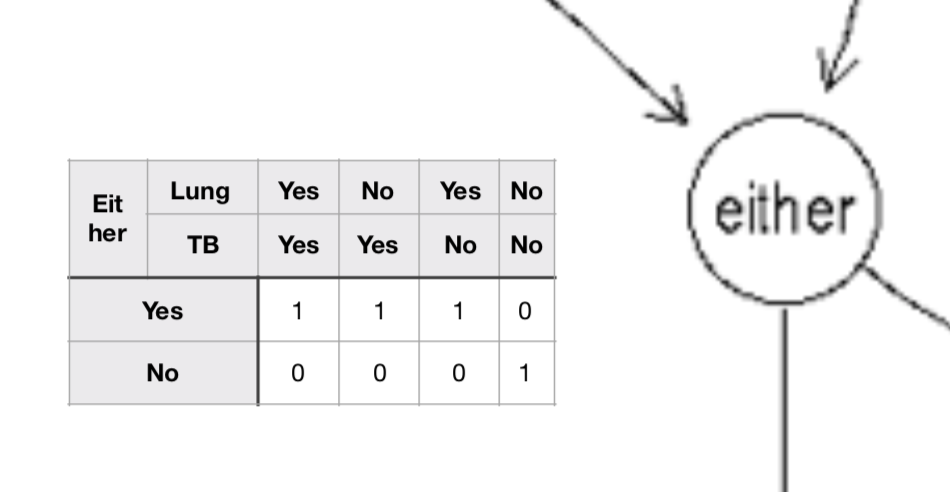
\includegraphics[width=0.4\textwidth]{pic/either01s.png}
            \caption{Node \textit{Either} from Asia Bayesian network}
            \label{fig:either01}
        \end{figure}
        
        \noindent After simplification, the clause generated by node \textit{Either}:\\
        \begin{center}
            $\neg \lambda_{Either_{yes}} \vee \neg \lambda_{Lung_{no}} \vee \neg  \lambda_{TB_{no}} $\\
            $\neg \lambda_{Either_{No}} \vee \neg \lambda_{Lung_{yes}} \vee \neg \lambda_{TB_{yes}}$\\
            $\neg \lambda_{Either_{No}} \vee \neg \lambda_{Lung_{No}} \vee \neg  \lambda_{TB_{yes}}$\\
            $\neg  \lambda_{Either_{No}} \vee \neg  \lambda_{Lung_{yes}} \vee \neg  \lambda_{TB_{no}}$
        \end{center}
        
        \noindent In paper \cite{enc2} proved that this simplification will lead to large reduction in the CNF sizes, the results are further discusses in \textcolor{red}{Section 7.3 Encoding deterministic}.\\
        
        \noindent \textbf{Weights assigning rules}:\\
        
        \noindent For each CNF literal, we need to assign a weight. These are the rules for assigning weights
        \begin{itemize}
            \item For both positive and negative indicator variables, assign weights to 1.
            \item For negative parameter variables, assign weights to 1.
            \item For positive parameter variables, assign weights that is the same as the parameter values in the CPTs.
        \end{itemize}
       
        For example, consider Nodes Aisa and Tub in Figure \ref{fig:asia-tub} and the clauses they generate. 
        \begin{center}
            $Weight(\theta_{asia_{Y}}) = 0.5$\\
            $Weight(\theta_{asia_{N}}) = 0.5$\\
            $Weight(\theta_{TB_{Y}}|Asia_{Y}) = 0.05$\\
            $Weight(\theta_{TB_{Y}}|Asia_{N}) = 0.01$\\
            $Weight(\theta_{TB_{N}}|Asia_{Y}) = 0.95$\\
            $Weight(\theta_{TB_{N}}|Asia_{N}) = 0.99$\\
        \end{center}
        The weight of the rest of the literals equals to 1. \\
        
        \noindent Now for each model, the weight of one model equals the product of all positive parameter variables. 
        $$\textbf{\textbf{W}} = \prod_{i = 0}^{n} Weight(\theta_{X_{n}}) $$
        The process to answer specific queries is to change the weight of variables with contradicting subscript to the indicators to 0.
        
        
        \subsubsection{Improved Encoding}
        Note: this encoding is done based on the Full encoding in section. 
        The idea is to use less clauses and variables to encode the CPT by encoding equal parameters. A key observation of the CPT is that using the Improved Full Encoding, no two parameter variables generated from the same CPT can be set as TRUE simultaneously, since their network instantiations are not consistent. \cite{enc2} proposed that within a CPT, if there are multiple \textbf{non-extreme} variables that has the same value, instead of generating new variables each time, we can use one logic variable to represent the parameter values.\\
        
        \noindent \textbf{\textit{Improved Encoding Steps:}}\\
        \textbf{Obtaining indicator clauses \textsc{I}:}\\
        For each node \textit{X} in a Bayesian Network with probability \{$x_{1}$,... ,$x_{n}$\} $\in$ \textit{X}, the following clauses are generated:
        \begin{equation}\label{Improvedenc_ic}
            \lambda_{x_{1}} \vee ... \vee \lambda_{x_{n}}
        \end{equation}
        This step is the same as the Full encoding.\\

        \noindent \textbf{Obtaining Parameter clauses \textsc{P}:}\\
        For each node \textbf{\textit{X}} in a Bayesian Network and its corresponding CPT:
        \begin{itemize}
            \item For \textbf{extreme parameter values} in the CPT, parameter variables are generated as the same way as the Simplification of  Full encoding.
            \item For each \textbf{non-extreme value} \textit{v}, we generate one parameter variable $\theta_{v}$.\\
        \textbf{Problem Raised:} Following the full encoding scheme, assume the following part from Node C with parent nodes A and B in a Bayesian network:
        %\begin{center}
        \begin{multicols}{2}
        [
        The following parameter clauses are generated
        ]
        
        \begin{center}
        \vspace{10mm}
            \begin{tabular}{ c c c c } 
            \hline
            C & A & B & P\\
            \hline
            \hline
            $C_1$ & $A_1$ & $B_1$ & 0.2\\
            $C_2$ & $A_2$ & $B_2$ & 0.2\\
            \hline
            \end{tabular}\\ 
        \end{center} 
        \columnbreak
            
        $\lambda_{a_{1}} \wedge \lambda_{b_{1}} \wedge \lambda_{c_{1}} \rightarrow \theta_{0.2}$\\
        $ \theta_{0.2} \rightarrow \lambda_{a_{1}} \wedge \lambda_{b_{1}} \wedge \lambda_{c_{1}}$\\
        $\lambda_{a_{2}} \wedge \lambda_{b_{2}} \wedge \lambda_{c_{2}} \rightarrow \theta_{0.2}$\\
        $ \theta_{0.2} \rightarrow \lambda_{a_{2}} \wedge \lambda_{b_{2}} \wedge \lambda_{c_{2}}$\\
        \end{multicols}
        
        %\end{center}
        For the value 0.2 in this table, $\theta_{0.2}$ is used for the parameter variable, we got $ \theta_{0.2} \rightarrow \lambda_{a_{1}} \wedge \lambda_{b_{1}} \wedge \lambda_{c_{1}}$ and $ \theta_{0.2} \rightarrow \lambda_{a_{2}} \wedge \lambda_{b_{2}} \wedge \lambda_{c_{2}}$ in the clauses. The $\theta_{0.2}$ implies incompatible configurations of the variables\cite{enc2}.  \\
        
        \textbf{Solution:} The solution given in \cite{enc2} is to replace the Full encoding \ref{fullenc_pc1} with the following clause:
        \begin{equation}\label{improvedenc_pc}
            \lambda_{x_{i}} \wedge \lambda_{y_{1}} \wedge... \wedge \lambda_{y_{m}} \rightarrow \theta_{x_{i}|y_{1}..y{m}}
        \end{equation}
        This introduced new models compared to the Full Encoding method in \cite{enc1}, while according to \cite{enc2}, the newly introduced model has larger cardinality and this can be solved by adding a condition when the output is fed into the model counter.\\
        
        \noindent\textit{ Thereom}\cite{enc2}: Consider a Bayesin network with n variables, the cardinality of the models for CNFs  generated by Full encoding (denoted by \textbf{A}) equals to 2n, the cardinality of the models for CNF generated by Improved encoding that are not in \textbf{A} is larger than 2n.\\
        Therefore, the unwanted models have a higher cardinality (/> 2n), by minimizing during model counting. we can drop the PI clauses defined in equaltion \ref{fullenc_PI} during the encoding process.
        \end{itemize}
        
        \noindent Use DP\%  to describe the percentage of remaining variables if we use the same variable to represent the same values within a CPT. \cite{2008-literature-review} showed that the reduction can be up to 95\% for some of the experimented networks.\\
        
        %%% Give an example here
        %Consider the node $\theta_{Dysp_{yes}|Bronc_{yes},either_{yes}} = 0.9$ and $\theta_{Dysp_{no}|Bronc_{no},either_{no}} = 0.9$,  If we follow the encoding method described in Full encoding, the following clauses are generated.
        \subsubsection{Group Encoding}
    
        The Improved Encoding discussed in \textcolor{red}{Section 3.2.3} gives an improvement of encoding Bayesian Networks by encoding equal parameter values. \cite{2006-enc3} proposed a method which use less variables by pre-processing the CNF to simplify the clauses.\\
        
        For each CPT, the rows which has the non-extreme values are partitioned into several groups based on the value. Within each group, we apply a simplification to try to reduce the number of variables and clauses inspired by the resolution strategy in boolean logic.\\
        
        In boolean logic, Consider two clauses $\alpha \vee \beta \vee \gamma$  and $\alpha \vee \neg\beta \vee \gamma$
        replace them with a single clause: $\alpha \vee \gamma$
        
        $$\frac{ \alpha \vee \beta \vee \gamma, \quad \alpha \vee \neg\beta \vee \gamma}{\alpha \vee \gamma}$$
        
        Within a CPT, we do the following process before generating parameter clauses:\\
        \begin{enumerate}
            \item Partition the CPT into groups based on non-extreme values, and the rows with extreme values remains the same.
            \item For each group of rows \textbf{R}, apply the Extended QM algorithm to simplify the clauses and variables with the clauses.\\
        \end{enumerate}
        
        
        Here's an example:\\
        \begin{table}[ht]
        \centering
        \begin{tabular}{c c c c}
            \hline
            \hline
            Dyspnea & Bronc & Either & Pr\\
            \hline
            \hline
            1 & 1 & 1 & 0.9 ($\theta_{1}$) \\
            1 & 0 & 1 & 0.9 ($\theta_{1}$)\\
            0 & 0 & 0 & 0.9 ($\theta_{1}$)\\
            0 & 0 & 1 & 0.1 ($\theta_{2}$)\\
            0 & 1 & 1 & 0.1 ($\theta_{2}$)\\
            1 & 0 & 0 & 0.1 ($\theta_{2}$)\\
            1 & 1 & 0 & 0.8 ($\theta_{3}$)\\
            0 & 1 & 0 & 0.2 ($\theta_{4}$)\\
            \hline
        \label{table:nyspnea_asia}
        \end{tabular}
        \caption{CPT of node Dysnpea from Asia Network}
        \end{table}
        
        \begin{multicols}{2}
        \centering
        \noindent Improved encoding:\\
        $Dyspnea_{1} \vee Bronc_{1} \vee Either_{1} \rightarrow \theta_{1}$\\
        $Dyspnea_{1} \vee Bronc_{0} \vee Either_{1} \rightarrow \theta_{1}$\\
        $Dyspnea_{0} \vee Bronc_{0} \vee Either_{0} \rightarrow \theta_{1}$\\

        \columnbreak
        
        \noindent simplify the clauses\\
        $Dyspnea_{1} \vee Either_{1} \rightarrow \theta_{1}$\\
        $Dyspnea_{0} \vee Bronc_{0} \vee Either_{0} \rightarrow \theta_{1}$\\
        \end{multicols}
        Consider the table \ref{table:nyspnea_asia}. Given values to some of the variables, some other variables will become irrelevant, so that it allows the clauses to be simplified. Since Bayesian network variables may have cardinality larger than 2, the resolution for boolean variables were extended for multi\-variate variables.\\
        
        \cite{2006-enc3} defined a sytax for multiple variable logic:
        \begin{itemize}
        \item An atom is an assignment to a variable in \textbf{X} of a value in the domain.
        \item A \textit{world} that consits of an atom for each variable, satisfy an atom if and only if it assigns the common variable the same value
        \item A term over $\textbf{X}' \subseteq \textbf{X}$ is a conjunction of atoms.
        \item $\Gamma$ is a disjunction of terms over X.
        \item An \textit{implicant} $\gamma$ of $\Gamma$ is a term over \textbf{X'} $\subseteq$ \textbf{X} that implies $\Gamma$.
        \item A \textit{prime implicant} is an implicant that is minimal when the removal of any atom will cause in a term that is no longer an implicant of $\Gamma$.
        \end{itemize}
        
       In boolean logic, QM algorithm aims to simplify Boolean functions. The algorithm was developed by Willard V. Quine and extended by Edward J. McCluskey.\\
        
        In order to generate prime implicants for Bayesian Network variables, the QM algorithm need to be extended. In \cite{2006-enc3}, the paper cited was not found so I extended the QM algorithm in a straightforward way and will be discussed in seciton \textcolor{red}{4.7.2}
        
        \subsubsection{Cachet Encoding}
        The Cachet encoding we are refereing to is based on the encoding presented in \cite{Sang:2005:PBI:1619332.1619409}. One of the assumption in this encoding is that there's an ordering on the values for each network variable. We call $x_{i} < x_{j}$ if $x_{i}$ comes earlier in the variable value.\\
        
        Cachet Encoding provide same indicator variables as Full encoding. For the parameter in a nerwork Pr($x|Y$), when x is not the latest value in X, define a parameter variable $\rho_{x|Y}$.
        
        Then the Cachet encoding \textbf{define the CNFs}: Cachet encoding generate the same indicator clauses as Full encoding. For each network variable, Cachet encoding provide the following clauses for parameter value $Pr(x_{i}|y_{1}, ... , y_{m})$.
        \begin{itemize}
            \item If x is not X's last value: $$\lambda_{y_{1}} \wedge ... \wedge \lambda_{y_{m}} \wedge \neg \rho x_{1|Y} \wedge \neg \rho x_{i-1|Y} \wedge \rho_{x_{i}|Y} \rightarrow \lambda_{x_{i}}$$
            \item If x is X's last value:
            $$\lambda_{y_{1}} \wedge ... \wedge \lambda_{y_{m}} \wedge \neg \rho x_{1|Y} \wedge \neg \rho x_{i-1|Y} \rightarrow \lambda_{x_{i}}$$
        \end{itemize}
        \subsubsection{Log-encoding}
        In \cite{2016-logencoding}, the author proposed an Encoding scheme based on the Group Encoding method. There are two key steps in this encoding. First, a logarithm encoding to define indicator variables. Second, a scaling factor within each CPT to scale the weight assigning.\\
        
        \noindent First consider the logarithm encoding, this step is similar to the binary encoding. For a node with N indicator variables, $\lceil N \rceil$ of propositional variables are used to represent the indicator variables. Table \ref{tab:log_example} shows an example log encoding.\\
        \begin{table}[]
            \centering
            \begin{tabular}{c l}
                \hline
                \hline
                Node Variables	&	Encoded clauses	\\
                \hline
                $X_{1}$	&	$\neg c_{0} \wedge \neg c_{1}$	\\
                $X_{2}$	&	$\neg c_{0} \wedge c_{1}$	\\
                $X_{3}$	&	$ c_{0} \wedge \neg c_{1}$	\\
                \hline
                Exclude extra enc: & $c_{0} \vee  c_{1}$\\
                \hline
                \hline
            \end{tabular}
            \caption{An example log encoding of indicator variables}
            \label{tab:log_example}
        \end{table}
        
        \noindent The notation for encoded indicator clauses in \cite{2016-logencoding} is $\tau((X, d))$, in which \textit{X} is the set of propositional variables and \textit{d} indicates which propositional variable is positive in the clauses. For each parameter clauses, we have the following two kinds of situations:
        
        \begin{itemize}
            \item If the parameter value Pr($\theta_{m}$) = 0: $\bigvee \neg \tau(X, d)$ 
            \item If the parameter value Pr($\theta_{m}$) $\neq$ 0: $\bigvee \neg \tau(X, d) \vee \theta_{m}$ 
        \end{itemize}
        
        Then we consider the weight assigning rules. After multi-variable simplification is performed within a CPT, select the remained non-zero parameter $\theta_{j}$ that is the most frequent as the scaling factor for the weights, and use $W_{\theta_{j}}$ to denote the scaling variable. For all parameter vairiable $\theta_{i}\; i \neq j$, 
        $$W(\theta_{i}) = \frac{OriginalWeight(\theta_{i})}{W(\theta_{j})}$$
        For negative parameter variables:
        $$W(\neg \theta_{i}) = 1 - W(\theta_{i})$$


    \subsection{Exact Model Counters}
    There are mainly two types of weighted model counting methods, Search-based methods and Compilation-based methods. This section mainly compares three typical model counting methods called Cachet \footnote{cachet link: http://www.cs.rochester.edu/u/kautz/Cachet/index.htm}, C2D \footnote{C2D link: http://reasoning.cs.ucla.edu/c2d/}, and Ace \footnote{Ace link: http://reasoning.cs.ucla.edu/ace/moreInformation.html}.
    \subsubsection{Search based model counter}
    \textbf{Cachet:}\\
    In \cite{Bayardo:2000:CMU:647288.721114}, the author showed that a Conjunctive Normal Form can be decomposed into components such that no two components share same variables
    so that the models can be counted by counting each component independently.
    Search based model counter count models by forcing decomposition. The process is described below:
    \begin{enumerate}
        \item Perform splitting on some variables
        \item Perform Unit resolution
        \item Do 1 and 2 for the sub component generated so far recursively 
    \end{enumerate}
    An example is given in \cite{2008-literature-review}. Consider the set of clauses:\\
    \begin{center}
        $A \vee B \vee C$\\
        $A \vee D \vee E$\\
        $\neg A \vee \neg B \vee C$\\
        $\neg A \vee \neg D \vee E$\\
    \end{center}
    
    The Figure \ref{fig:searchfig} shows the result after splitting.
    
    \begin{figure}
        \centering
        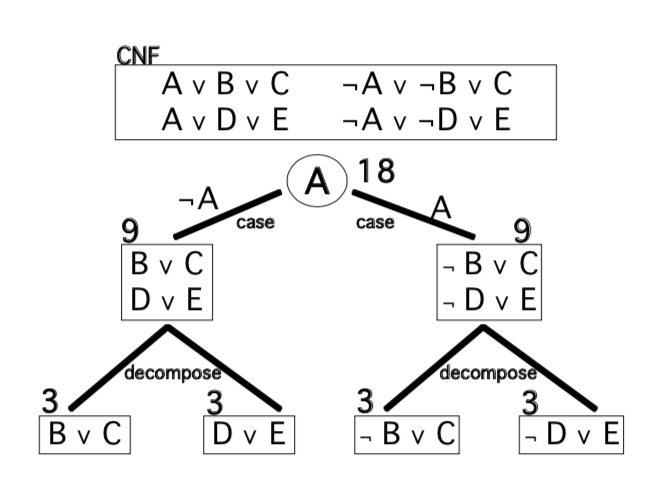
\includegraphics[width = 0.5 \textwidth]{pic/searchalgo.png}
        \caption{The illustration of search based algorithm to perform model counting from \cite{2008-literature-review}}
        \label{fig:searchfig}
    \end{figure}
    
    Compared to the Compile-based model counters, model counters by searching require less computational space. One of the most widely search\-based model counter is called cachet proposed in \cite{Cachet}, combined with the encoding method we discussed in \textcolor{red}{1.2.5 Cachet Encoding}, it showed strong ability to perform probabilistic inference and the result was demonstrated in \cite{Sang:2005:PBI:1619332.1619409}\\
    
    \noindent \textbf{SharpSAT:}\\
    Similar to Cachet, the SharpSAT first proposed in \cite{Sharp-SAT2006} used the DPLL algorithm \\
    Some of the algorithms such as \textcolor{red}{DPLL with caching: a NEW ....} improved the performance using techniqes such as Component Caching
    \subsubsection{Compile based model counter}
    Another categrory of model counter use knowledge compilation, which the process aims to compile one type logic form into another one.\cite{2008-literature-review} In \cite{2002language-map}, a \textit{represented language} (such as CNF) is defined as sth we expect human to read and write without too much effort, and the \textit{target compilation langauge} are in the form such that it can repond queried in poly\-time. Some of the widely used compile\-based model counters are C2D and miniC2D.\\
    
    \textbf{C2D}:\\
    C2d was deveploped by \textcolor{red}{UCLA Reasoning group}. In \cite{c2d}, the CNF of a Bayesian network, encoded using Full Encoding discussed above, was compiled in to d\-DNNF, and this is a form of knowledge representation knowledge that support model counitng in poly\-time to the size of the input compiled form (d\-DNNF) \cite{2002language-map}.\\
    
    Model counting require three property, decomposition, determinism, and smoothness which is satisfied by d\-DNNF. Compiling CNF into d\-DNNF will support weighted model counting by traversing the d\-DNNF and multiply or add the results.\\
    
    \textbf{mini-C2D}:\\
    The model counter mini\-C2D was proposed in \cite{minic2d}. Minic2d is a top\-down compiler that given the CNF clauses as input, it compile the CNF into Sentential Decision Diagram (SDD).\\
    
    One of the main disadvantages is that the compiled file size can be larger than the available memory, futher results are shown in the Results and analysis in \textcolor{red}{Section 7.6}.
    
    \subsection{Selection and decision}
    In this project, I implemented the encoding schemes including Full encoding, Simplified Full encoding, Improved encoding and Group encoding, and I used the miniC2D for model counting. \\
    
    The four encoding schemes are closely related to each other and perform improvement step by step. Thus, it is more fair to compare the performance during the model counting phase.\\
    
    The model counting tool is miniC2D. The model counting tool is can be run cross platform under both macOS and linux. The weight is formatted in a simpler way in one line compared to other available model counters. In addition, according to \cite{minic2d}, the performance is among the best.\\
    
    In \cite{2008-literature-review}, the combining of the four encoding schemes and compiled based model counters give strong performance and good results. It is reasonable to expect the newer model counter miniC2D can perform equally strong for the benchmark problems.
    
    % \subsubsection{Cachet and C2D model counter}
    % Cachet is a search based model counter \cite{Cachet}. The idea behind is to decompose the CNF clauses into several components that does not share variables, so that each component can be counted separately. When all the clauses share some same variables, splitting is required to force the decomposition. \\\par
    % Compared to some of the model counter that explore  topological structure, Cachet performed better in the experiment in \cite{2008}.\\\par
    % C2D \cite{c2d} is a knowledge compiler that is based on a search based model counter, while it keep trace of its operations, and it also use a different method to implement decomposition, variable splitting and caching.
    % \subsubsection{Ace model counter}
    % Ace \cite{Ace} is a knowledge compilation based model counter that compile one logical form into another target logical form. For example, in section 2.1.1, after encoding the Bayesian Networks into CNF using Encoding 1, The CNF need to be compiled into d-DNNF. The d-DNNF supports model counting in polytime in the size of the compiled form.
    


\newpage
\section{Design and Implementation}
This section is dedicated to explaining the language and library used in implementation, an extension of the library method, and the implementation of the chosen encoding schemes and three key storage used in the encoding.

    \subsection{Programming Language}
I used \textbf{Python} for the implementation. Although python programs are generally expected to run slower than some other Object-oriented programming languages like JAVA and C++, it enables the programs to become three to five times shorter than JAVA and five to ten times shorter than C++.\footnote{https://www.python.org/doc/essays/comparisons/}, 
and Python also supports powerful dictionary and list types. \\

\noindent Another reason for using Python is that with certain libraries, Bayesian Networks can be imported or defined in a simple way, so that it supports testing the performance with widely used benchmarks.

\subsection{Input format}
The input is the \textbf{Bayesian Interchange Format} (BIF) which are files with .bif extension to represent Bayesian Networks. The BIF files are used as input because it's a widely used format in tools that are dealing with Bayesian Networks including BayesiaLab \footnote{http://www.bayesia.com/}, JavaBayes\footnote{https://www.cs.cmu.edu/~javabayes/Home/} etc, so there are a lot of available benchmarks with the BIF Format. In general, Four types of blocks are defined.\\

\noindent \textbf{The Network Block:}\\
\noindent A network block defines the name of the network and lists the properties. The example below specify the network block for the Asia Bayesian Network:
\begin{lstlisting}
network asia{
  property version 1.1;
  property author ..;
}
\end{lstlisting}

\noindent \textbf{The Variable Block:}\\
Variable blocks define the variables in a network. These blocks used
to be called node blocks in the BIF; it seems that variable conveys
more of a statistical meaning while node just refers to a graphical
concept. The example below is the bronc node from asia.bif
\begin{lstlisting}
 variable bronc{
    type discrete [2] {yes, no};
 }
\end{lstlisting}

\noindent \textbf{Blocks for standard nodes}\\
Standard nodes have to define the probabilities for each discrete parent instantiation. An example of a standard probability block is: 
\begin{lstlisting}
 probability (dysp | bronc, either){
    (yes, yes) 0.9, 0.1;
    (no, yes) 0.7, 0.3;
    (yes, no) 0.8, 0.2;
    (no, no) 0.1, 0.9;
}
\end{lstlisting}

\noindent \textbf{Probability blocks}:\\
Probability blocks are another way to specify the (conditional) probability tables (CPTs). For these variables, and hence the topology of the network. The block indicates the variables of the probability distribution right after the keyword probability.
\begin{lstlisting}
probability (v_10_8 v_10_7 v_9_8){ 
table 0.586357 0.667473 0.789088 0.466932 
      0.413643 0.332527 0.210912 0.533068;
}
\end{lstlisting}
A more detailed explanation of the BIF is explained here: \footnote{http://www.cs.washington.edu/dm/vfml/appendixes/bif.htm} \\

\subsection{Output}
The output of the program is the cnf file following the DIMACS format which is a widely accepted standard format for representing CNF clauses and it's also the input format used by most of the model counters mentioned in section 3.3.\\
\begin{itemize}
    \item A comment line starts with a \textit{c}
    \item A line p cnf var clauses specify the instance in CNF format, in which \textit{vars} is the number of variables used in the file and \textit{clauses} is the number of clauses in the CNF.
    \item Each CNF variable is denoted by a non\-zero number smaller than \textit{vars}, the negation of a variable is denoted by a negative number.
    \item Each clauses contains one or several CNF variables, 0 specifies the end of the clause.
\end{itemize}

Consider the following CNF:
\begin{center}
    $x_{1} \vee x_{2} \vee \neg x_{3}$\\
    $x_{1} \vee x_{4} \vee x_{5}$\\
    $\neg x_{3} \vee \neg x_{4}$\\  
\end{center}
The clauses in DIMACS format:
\begin{center}
    \begin{lstlisting}
    c A sample DIMAC file
    p cnf 5 3
    1 2 -3 0
    1 4 5 0
    -3 -4 0
    \end{lstlisting}
\end{center}
    
\subsection{Pgmpy}
The library to read and represent Bayesian networks is Pgmpy \cite{pgmpy_paper}. With Pgmpy, Bayesian network can be easily created, and it also support reading Bayesian networks from BIF format. The library is opensource so that it can be modified and extended if required. Pgmpy also have build-in inferencing method using Variable Elimination so that the run time can be used to evaluate the performance. 

 \subsection{Extend the Pgmpy library}
    Pgmpy library does not support fetching CPT values using table indexing, the only way to fetch value is through specifying evidence and variables and query the value through Variable Elimination method. The Variable Elimination method is the bayesian inference method that is \textcolor{red}{Insert time complexety}. To solve the problem, I extended the pgmpy library to support fetching variable values without querying using Variable Elimination.\\

    \noindent \textbf{The TabularCPD Class}:\\
    The method get\_cpds returns a conditional probability distribution of the node, the returned type is defined as TabularCPD that contains the name of the node, cardinality, variables which are stores as a nested list, the list of evidences and their corresponding cardinalities. An example is given below:
    \begin{lstlisting}
    cpd = TabularCPD('dysp', 2, [[0.9, 0.7, 0.8, 0.1],
                                 [0.1, 0.3, 0.2, 0.9]],
                                 ['bronc', 'either'], [2, 2])
    \end{lstlisting}

    \noindent \textbf{The storage of a TabularCPD}:\\
    calling cpd.variables() will return a list starts with the node variable followed by the the evidences, and calling cpd.cardinality() will return the cardinality list in the same order as the variables returned by cpd.variables()
    \begin{lstlisting}
    >> print(cpd.variables())
        >> ['dysp', 'bronc', 'either']
    >> print(cpd.cardinality())
        >> ['2', '2', '2']
    \end{lstlisting}

   \noindent \textbf{MyCPD}:\\
    col\_index stores the index of the combination of evidence, in the same order as the probability distribution defined in the \textbf{standard node block}. The col\_index is constructed using the itertools.product in python which return the cartesian product. The transpose of the col\_index correspond to the order of the probability distribution specify in the BIF file. Consider the example with node \textit{dysp}.
    \begin{lstlisting}
    >> col_indexes = np.array(list(product(*[range(i) for i in ev_card])))
    >> print(evidence, col_index) 
        >> ['either', 'bronc']
        >> [[0 0]
            [0 1]
            [1 0]
            [1 1]]
    \end{lstlisting}
   
    \noindent Then the evidences are formatted into tuples with the same length and each column correspond to one entrance to the probability table.\\
    \begin{lstlisting}
    A sample return the evidence entrance. 'dysp' node in aisa.bif
    >> entrance <- [('{s}'.format(s = reverse_ev[i]), d) 
                    for d in col_indexes.T[i]]
        >> [('either',0), ('either',0), ('either',1), ('either',1)]
           [('bronc', 0), ('bronc', 1), ('bronc', 0), ('bronc', 1)]
    Then the entrace are transposed using rol_to_col()
    >> rol_to_col(entrance)
        >> [[('bronc',0), ('either',0)], [('bronc',1), ('either',0)], 
            [('bronc',0), ('either',1)], [('bronc',1), ('either',1)]]
    \end{lstlisting}
    
    \begin{minted}
    [linenos]
    {python}
    Parameter: A TabularCPD
    def myCPD(TabularCPD cpd):
        var, evidence <- cpd.variable[0], cpd.variable[1:]
        var_card, ev_card <- cpd.cardinality[0], cpd.cardinality[1:]
        variable <- [(name, 0),.., (name, n)]
        value = cpd.values()
        # node with evidence:
        if evidence not null:
            col_indexes <- get index
            for i in cardinality:
                entrance <- format the header
                rol_to_col(entrance) # transpose
            for each node variable:
                newcpt.append(variable, index, evidence, corresponding_value)
        # node with no evidence
        else:
            for each node variable
                newcpt.apend(variable, index, [], corresponding_value)
    \end{minted}
    A Sample return of newcpt of node dysp:
    \begin{lstlisting}
    [('dysp', 0, [('bronc', 0), ('either', 0)], 0.9), 
     ('dysp', 0, [('bronc', 1), ('either', 0)], 0.7), 
     ...
     ('dysp', 1, [('bronc', 0), ('either', 1)], 0.2), 
     ('dysp', 1, [('bronc', 1), ('either', 1)], 0.9)]
    \end{lstlisting}
    The method mycpd(TabularCPD) returns a table\-like list of tuples, the first two element in each tuple forms the node variables and the third element is a list of evidence. An example of the first tuple in the list means $dysp_{0}|bronc_{0}either_{0} = 0.9$. Now the returned data support fetching values using list indexing so that we don't need to query the value using the time-consuming Variable Elimination.\\ 
    
    
    \noindent In our case for both bronc and either, the evidence all equals to 2, the convention for the order is shown in figure \ref{fig:sample print table}. The list which store the values are the transpose of the matrix in BIF format.\\
    \begin{figure}
        \centering
        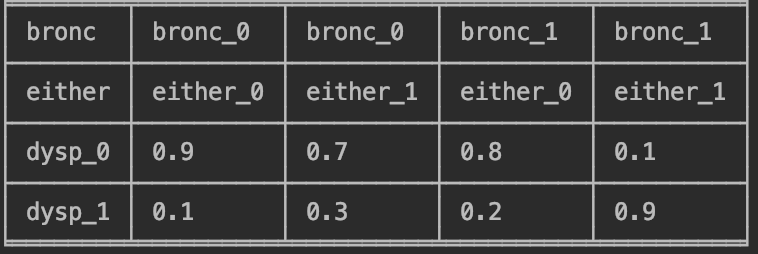
\includegraphics[width = 0.7\textwidth]{pic/printBayesnode.png}
        \caption{A sample printed CPT of a node dyps}
        \label{fig:sample print table}
    \end{figure}
    
\subsection{Storing variables, weights and CNFs}
There are three important storage in the implementation, the generated variables, corresponding weights and the representation of CNFs.\\

\noindent Variables in the CNFs and its corresponding weights are stored in python dictionaries. One of the consideration is the speed of looking up  a certain variable weights or its corresponding integer used in the DIMAC format. Encoding Bayesian networks might lead to dealing with large number of variables. Some of the results \cite{2008-literature-review} shows that the variable numbers might reach over 50,000. \\

\noindent If we use a list of pairs to store the variables or the weights, the time complexity for looking up a list is \textbf{O}(n) for linear search over the list. However, the time complexity for looking up in the dictionary is \textbf{O}(1). When dealing with large number of variables, the time difference is substantial. In addition, adding the dictionary operation 'add' is an process with O(1) regardless of the size of the dictionary. The key in the variable is the name of the variable, \textit{weights} stores its corresponding weight and the var\_dic stores the integer used to represent the variable in the DIMAC format.

\begin{lstlisting}
var_dic = {
    'theta_x1|y1y2': 5,
    ...
}

weights = {
    'theta_x1|y1y2': 0.03,
    ...
}
\end{lstlisting}

\noindent The CNF clauses are stored as a list of lists. Inner list represent one clause that are the disjunction of literals, and the outer list represent the conjunction of the clauses. We use list to store the clauses because once a clause is generated and append to the list, it won't be modified during the later process, and no other operation such as list lookup is needed. The only operation is to traverse each clause in the list that the CNF to write to files.

    \subsection{Implementation of Full encoding}
    In section 3.1 Full encoding, for each node in the Bayesian network, two kinds of variables need to be generated, indicator variables and parameter variables respectively. This section will first show the steps to generate indicator variables and indicator clauses and then show the steps to encode parameter variables and clauses.
    \begin{itemize}
        \item \textit{var\_dic} is a dictionary in which the key is the name of the variable and the value is used when the cnf is written into the DIMACS format. 
        \item \textit{clauses} is a nested list, each element correspond to one clauses in the generated CNF. Literals are stores as a tuple (sign, variable). sign = -1 means the negation of the variable
        \item \textit{weights} is a dictionary that stores the corresponding weights of the variable following the weights assigning rules mentioned in section 3.2.2. The key is the name of the variable such as $\lambda_{dysp_{0}}$ and the value is the corresponding weight.
    \end{itemize}
    \textbf{Generating Indicator variables:}\\
    Given a bayesian network \textit{bn}, for each node in the network, define the number of indicators same as its cardinality. Then two types of clauses are generated: $[\lambda_{x_{1}}, ... \lambda_{x_{n}}]$ and $[\neg \lambda_{x_{i}}, \neg \lambda_{x_{j}}]$ when $i < j$. weights($\lambda_{x}$) = 1, weights($\neg \lambda_{x}$) = -1. Traverse the node in the given Bayesian network and all indicator clauses are generated.
    The Psuedocode for generating indicator variables and clauses is given below:
    \begin{minted}
    [linenos]
    {python}
    def indicator(bn, var_dic, clauses, weights):
        for i in bn.nodes:
            cardinality <- bn.get_cardinality(i)
            # get variables
            for j in range(cardinality):
                name <- 'lambda_' + str(i)+ '_' + str(j)
                # append variable to variable dictionary
                # store the corresponding weights
                if name not in var_dic:
                    var_dic[name] = max(var_dic.values()) + 1
                    weights[name] = 1
            # get clauses:
        for i in bn.nodes:
            cardinality <- bn.get_cardinality(i)
            cl = [] # cl store each clause in the CNF, represented by a list of tuples
            for j in range(cardinality):
                variable <- fetch the corresponding variable from the dictionary
                cl.append((1, variable)) # 1 represent positive
            clauses.append(cl)
            
            for m in range(cardinality):
                for n in range(m + 1, cardinality):
                    var1, var2 <- fetch lambda_i_n, fetch lambda_i_m
                    cl = [(-1, var1), (-1, var, var2)]
                    clauses.append(cl)
                    weights[m] = -1
    return clauses, var_dic, weights
    \end{minted}
    
    \noindent \textbf{Generating Parameter variables:}\\
    For each variable of a node in the bayesian network, first get the evidence of the variable and the the evidences' cardinality. These, together with the node's cardinality, specify the number of values in a conditional probability table. For each value, a parameter variable $\theta_{node_{i}|evidences}$ is generated.\\
    $$number\_of\_values = cardinality(node) \times \Pi_{i = 1}^n cardinality(evidence_{i})$$
    
    The corresponding clauses: (described in line 20 \~ 26 in psuedocode)
    \begin{itemize}
        \item $ \neg\lambda_{x_{i}} \vee \neg\lambda_{y_{1}} \vee... \vee \neg\lambda_{y_{m}} \vee \theta_{x_{i}|y_{1}..y_{m}}$
        \item  $\neg\theta_{x_{i}|y_{1}..y_{m}} \vee \lambda_{x_{i}}$
        \item $\neg\theta_{x_{i}|y_{1}..y_{m}} \vee \lambda_{y_{j}} \;\; \mbox{ j = 1, ..., m}$
    \end{itemize}
    
    \begin{minted}
    [linenos]
    {python}
    def parameter_cl(bn, var_dic, clauses, weights):
        for i in bn.nodes:
            cardinality = i.get_cardinality()
            evidence = i.get_evidence()
            if no evidence:
                for j in cardinality:
                    name <- theta_ij
                    var_dic[name] <- max(var_dic.value()) + 1
                    weight[name] <- fetch weight
                    clauses.append([(-1, var_dic['lambda_i']), (1, var_dic[name]])
                    clauses.append([(-1, var_dic[name]), (1, dic['lambda_i'])])
            else:
                ev_cardinality <- [ev.cardinality() for ev in i.evidence]
                evidence_lst <- generate evidence list()
                for j in cardinality:
                    for ev in evidence_lst:
                        name = 'theta_' + i + str(j) + '|' + ev
                        var_dic[name] <- max(var_dic.value()) + 1
                        weight[name] <- fetch weight
                        clauses.append([(-1, var_dic['lambda_i']),
                                        ...
                                        (-1, var_dic['lambda_evidences']),
                                        (1, var_dic[name]])
                    clauses.append([(-1, var_dic[name]), (1, dic['lambda_i'])])
                    ...
                    clauses.append([(-1, var_dic[name]), (1, dic['lambda_evs])])
        return var_dic, clauses, weights
    \end{minted}
    % \caption{Psuedocode for encoding parameter clauses}
    % \label{code:Full enc parameter clauses}

    \subsection{Simplified Full encoding}
    In simplified Full encoding, one of the main improvement is to capture the extreme values when generating the parameter clauses. Before generating variables and clauses, the weight is fetched from the Probabilty table.\\
    \newline
    \noindent If Pr($variable_{i}|evidence_{1}...evidence-{m}$) = 0, the parameter clauses won't be generated, and only one clause will be appended to the CNF: [$\neg \lambda_{variable_{i}|}, \neg \lambda_{evidence_{1}}, ..., \neg \lambda_{evidence_{m}}$].\\
    
    \noindent If Pr($variable_{i}|evidence_{1}...evidence-{m}$) = 1, no action is done and the program should move to the next entry of the probability table.\\
    
    \noindent The psuedocode for simplifying extreme values with evidence list not empty is given below, the case without evidence can be implemented similarly.
    \begin{minted}
    [linenos]
    {python}
    for i in bn.nodes:
        for j in i.get_cardinality():
            evidence = i.get_evidence()
            # case with evidence:
            if evidence not null:
                parameter_value <- fetched weight
                if parameter_value == 0:
                    clauses.append([(-1, var_dic[lambda_ij]),
                                    (-1, var_dic[lambda_evidence1]), 
                                    ... ,
                                    (-1, var_dic[evidence_m])])
                if parameter_value == 1:
                    continue
                else: 
                    do the same as Full encode parameter clauses
        
    \end{minted}
    According to \cite{enc1}, the simplification step lead to significant improvement in the number of clauses which directly influence the time and space usage in the model counting phase. Detailed result is discussed later in the Result section.
    
    \subsection{Implementation of Improved Encoding}
    The idea of Improved encoding is to use same logic variable to encode the parameter variables that have the same value in the CPT. For each node in the Bayesian network, the table is first partitioned in to several sub-tables based on the non-extreme probability values. This can be done with the sorting within the table fetched by myCPD(TabularCPD) method. After the partition of the table, an encoding scheme for paramter values and clauses is described.
    
    \subsubsection{Encoding each parameter value}
    If the value is unique or extreme (0 or 1), it's considered a subgroup itself. For each subgroup, let \textit{p} denotes each row in the subgroup, the following algorithm describes the encoding step for each subgroup.
    \begin{algorithm}
    \caption{Improved Encoding for each subgroup}\label{algorithm:encode group}
    \begin{algorithmic}[1]
    \Procedure{$Subgroup\_encode$}{$sub\_group$, $clauses$}
    \For{$each sub-group \tau $}
    \State $P \gets$ each row \textit{p} in subgroup \Comment{Assume $x_{1}, ev_{1}, ..., ev_{m}$ in p}
        \State \textbf{I} $\gets$ lambda\_xi, lambda\_ev1, .. lambda\_evm
            \Comment{I $\gets$ encodes p}
        \For{each p}
            \If {$\theta = 0$}
                \State continue
            \EndIf
            \If {$\theta = 1$}
                \State $clause \gets \neg I$
                \State clauses.append(clause)
            \Else
                \State $clause \gets \neg I \vee \theta_{index}$
                \State clauses.append(clause)
            \EndIf
        \EndFor
    \EndFor
    \State \textbf{return} $clauses$
    \EndProcedure
    \end{algorithmic}
    \end{algorithm}
    \subsection{Implementation of Group Encoding}
    \subsubsection{QM algorithm}
    QM algorithm, proposed by Quine and McClusckey, is an algorithmic way of simplifying Boolean logic functions. The library for QM algorithm applied for binary variables were used and extended to support the simplification for multi-variables.
    
    \subsubsection{An extension of QM algorithm for multi-variate simplification}
    To simplify multi\-variate Bayesian network variables, the QM algorithm were extended.\\
    
    \noindent For the variables in the CPT, a fixed length of bit string is used to represent the combination of variable. The length of bit string depends on the cardinality of each variable. 
    $$total\_length = \Sigma_{i = 1}^{m} \lceil log_{2}(Cardinality(Var_{i}))\rceil$$
    The bit string is then transformed from binary to decimal numbers as the input of QM algorithm. Then the output is spitted into small binary groups same as the length used to encode each variable. 'X' means the don't care case. If given values of for the other variables, the variable contains the don't care case will have a uniform probability or irrelevant, variable can be removed from the clause. Table \ref{tab:QM encode} gives and example for the extension. \\
    
    \begin{table}[]
        \centering
        \begin{tabular}{c c c c |c c}
            \hline
            Dysp & Bronc & Either & Pr & bitstring & decimal \\
            \hline
            \hline
             1 & 1 & 1 & 0.9 & 111 & 7 \\
             1 & 0 & 1 & 0.9 & 101 & 5 \\
             0 & 0 & 0 & 0.9 & 000 & 0 \\
            \hline
            card = 2 & card = 2 & card = 2 & -- & -- & -- \\
            \hline
        \end{tabular}
        \caption{An example of encoding using dysp node in asia.bif}
        \label{tab:QM encode}
    \end{table}
    
    \noindent This extension of the QM algorithm won't simplify the clauses into the most essential prime implicants for variables with cardinality $\>$ 2, while it the simplification of the encoding result already lead to significant improvement into number of clauses.\\
    
    \noindent Smaller clauses may be generated if we apply the algorithm multiple times while the runtime of QM algorithm is exponential to the size of variables. Therefore, the algorithm is only applied once for each subgroup of the CPD.\\
    
    \begin{lstlisting}
    An example process using the table mentioned above
    >> bitstring(table)
    >> qm.qm(ones = [0, 5, 7])
        >> ['000', '1X1']
    >> split_result(['000', '1X1'])
        >> [['0', '0', '0'], ['1', 'X', '1']]
    >> decode_qm_output -> [[Dyspnea_0, Bron_0, Either_0],
                            [Dyspnea_1, Either_1)]]
    \end{lstlisting}
    
    \noindent The output of the extendedQM(subgroup) is the simplified implicants of the subgroup. For each output, the following encoding steps are used to generated clauses:
    
    \begin{algorithm}
    \caption{Group Encoding for each subgroup}\label{algorithm:group encoding}
    \begin{algorithmic}[1]
    \Procedure{$Subgroup\_encode$}{$sub\_group$, $clauses$}
    \For{each sub-group $\tau$}
        \State P $gets$ output simplified groups from the extendedQM
        \State  I $gets$ lambda\_x1 , ... ,lambda\_evidence
        \For{each p}
            \If {$\theta = 0$}
                \State continue
            \EndIf
            \If {$\theta = 1$}
                \State $clause \gets \neg I$
                \State clauses.append(clause)
            \Else
                \State $clause \gets \neg I \vee \theta_{index}$
                \State clauses.append(clause)
            \EndIf
        \EndFor
    \EndFor
    \State \textbf{return} $clauses$
    \EndProcedure
    \end{algorithmic}
    \end{algorithm}

  


\section{Project Management}
\subsection{Original plan}
\subsection{Time line}
\subsection{Git contribution}

\newpage
\section{Dependencies}

\section{Results and Evaluation}
\subsection{Experiment Setup}

\subsection{Variable elimination and bayesian with weighted model counting}
insert table here

\subsection{Number of Clauses}


\subsection{Model counting results}


\newpage
\section{Conclusion}

\medskip
\newpage
\printbibliography

\newpage
\appendix
\section*{How to run}
\subsection*{Encoding}

\subsection*{Running miniC2D}
To download the model counter, go to page \textcolor{blue}{http://reasoning.cs.ucla.edu/minic2d/download.php}\\
To run the model counter, go to the downloaded folder.
\begin{lstlisting}
$ cd bin/darwin
For model counting
$ ./miniC2D -c <path to the CNF file> - C
\end{lstlisting}
A sample output of Model Counting:\\
\noindent\rule{15cm}{0.4pt}
\begin{lstlisting}
CNF stats: 
  Vars=36 / Clauses=92
  CNF Time	0.000s
Constructing vtree (from primal graph)...Wrong cut! 2 1
Wrong cut! 3 2
  DONE
Vtree stats:
  Vtree widths: con<=4, c_con=44 v_con=4
  Vtree Time	0.003s
Compiling... DONE
  NNF memory      	11.5 KB
  Learned clauses      	1
Cache stats:
  hit rate   	43.8%
  lookups    	32
  ent count  	18
  ent memory 	0.9 KB
  ht  memory 	152.6 MB
  clists     	1.0 ave, 1 max
  keys       	4.1b ave, 8.0b max, 2.0b min
  Compile Time	0.000s
Saving compiled NNF to file... DONE
  Save Time       	0.001s
NNF stats:
  Nodes           	281
  Edges           	418
Post compilation
  Loading NNF from file... DONE
  Load Time       	0.000s
NNF stats:
  Nodes           	281
  Edges           	418
  Counting... 128 models / 0.000s
Total Time: 0.114s
\end{lstlisting}
\noindent\rule{15cm}{0.4pt}
\end{document}
